\documentclass[a4paper,11pt]{article}
\usepackage[T1]{fontenc}
\usepackage[utf8]{inputenc}
\usepackage{lmodern}
\usepackage{graphicx}
\usepackage{float} 
\usepackage[francais]{babel}
\usepackage{setspace}

\onehalfspacing


\title{\LARGE{Projet composants distribués}\\\bigskip \textbf{Morse Translator}}
\author{Guillaume LAROYENNE\\
   Informatique et réseau,\\
   ENSISA,\\
   2A\\
   \bigskip
   \texttt{guillaume.laroyenne@uha.fr}
   }
\date{\today}

\begin{document}

  \maketitle
  \begin{center}
  \large{Lien vers les sources du projet :} \texttt{https://github.com/LaroyenneG/Morse-Tranlator.git}\\[2cm]
  \textit{Version de java utilisé : \texttt{JDK 1.7.0}}
  \end{center}

  
      
  \newpage

\tableofcontents

\newpage

	\section{Présentation}
	\subsection{Description}
	
	
    \subsection{Aperçu}
    \begin{figure}[H]
    	\begin{center}
    		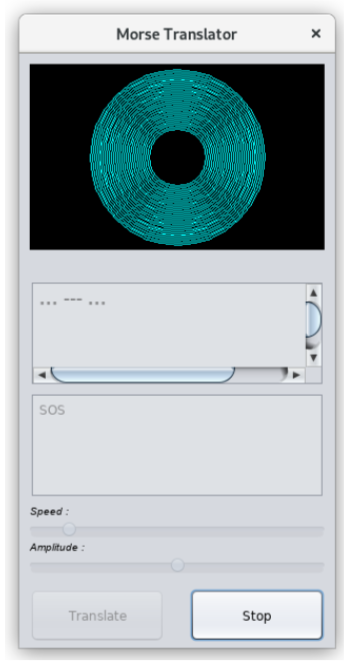
\includegraphics[scale=0.9]{descpicture.png}
    		\caption{Capture d'écran de l'application de test du composant}
    		\label{Capture d'écran de l'application de test du composant}
    	\end{center}
    \end{figure}
    
	\begin{figure}[H]
		\begin{center}
			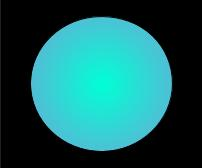
\includegraphics[scale=0.8]{comdescpicture.jpg}
			\caption{Interface graphique du composant}
			\label{Interface graphique du composant}
		\end{center}
	\end{figure}
    \subsection{Utilisation de l'interface de la démonstration}
    Pour utiliser l'interface vous devez entrer du texte dans la deuxième zone de texte. Une fois votre texte saisi vous pouvez appuyer sur le bouton "Translate". Le code Morse correspondant apparaîtra dans la première zone de texte. Vous pourrez également écouter et visualiser le signal correspondent en cliquant sur le bouton "play".\\
    \textbf{Attention} si vous modifiez les paramètres d'amplitude ou de vitesse vous devrez recliquer sur le bouton "translate" pour régénérer le nouveau signal analogique.
    

    \section{Modèle UML}
    \subsection{Diagramme d'états transitions}
     \begin{figure}[H]
    	\parshape1 -4cm 21cm
    	\begin{center}
    		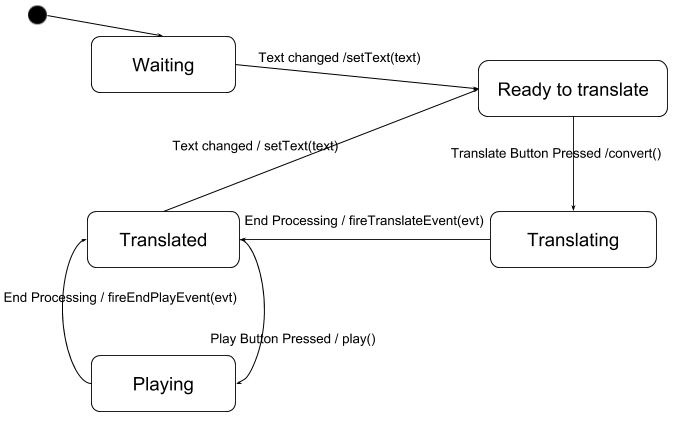
\includegraphics[scale=0.8]{etatsdiag.png}
    		\caption{Diagramme d'états transitions du composant}
    		\label{Diagramme d'états transitions du composant}
    	\end{center}
    	\parshape0
    \end{figure}
    \subsection{Diagramme des classes}
    \begin{figure}[H]
    	\parshape1 -4cm 21cm
    	\begin{center}
    		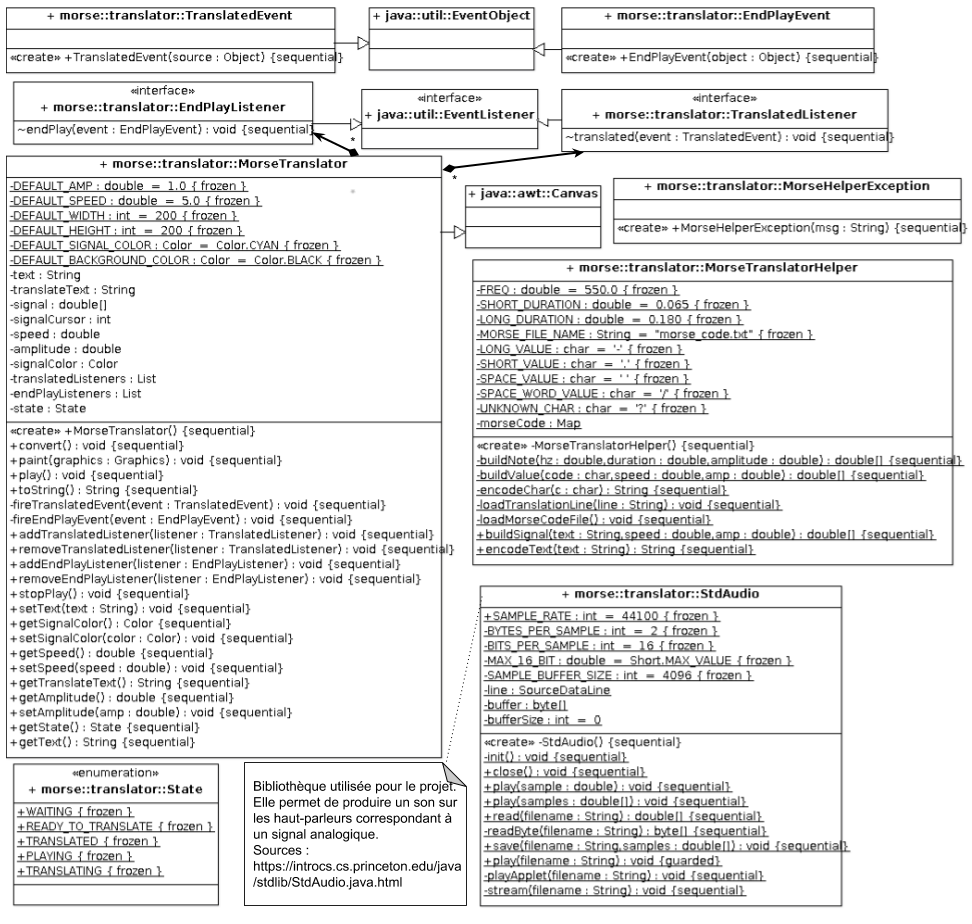
\includegraphics[scale=0.58]{classdiag.png}
    		\caption{Diagramme des classes composant}
    		\label{Diagramme des classes du composant}
    	\end{center}
   		\parshape0
    \end{figure}

\end{document}
